\subsubsection{06.04.15}
\begin{enumerate}
	
	\item The time of beginning and ending of the meeting: 16:10 - 21:50.
	
	\item Purposes of the meeting: 
	\begin{enumerate}
		
		\item To make MEL with transmission with gear ratio 2:1.
		
		\item To test new MEL.
		
        \item To fix MEL on the body of robot.
		
	\end{enumerate}

	\item Work that has been done:
	\begin{enumerate}
		
		\item New MEL was created and tested. Result is positive. Speed of lifting increased twice. But during the test threads that keep blocks torned. So it was decided to fix it by strong fishing cord. Today we didn't have time to fix The MEL on robot.
		\begin{figure}[H]
			\begin{minipage}[h]{0.47\linewidth}
				\center{
\includegraphics[scale=0.17]{days/06.04.15/images/01}}
				\caption{Testing new MEL}  
			\end{minipage}
			\hfill
			\begin{minipage}[h]{0.47\linewidth}
				\center{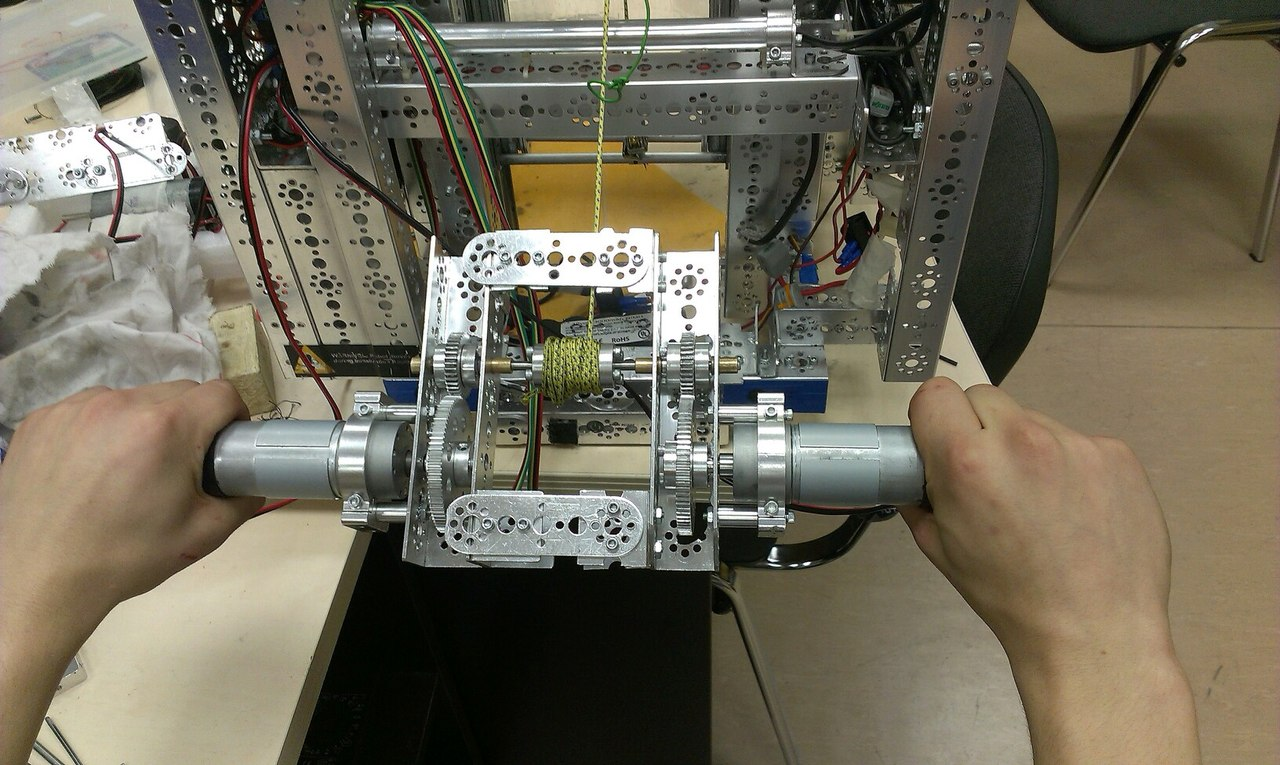
\includegraphics[scale=0.17]{days/06.04.15/images/02}}
				\caption{MEL's construction}
			\end{minipage}
		\end{figure}
		
		\item Also during the test we found that lift shakes when we rise it. It happend because rails extract not to maximal high. But we knew, how to solve this problem: install limiters which will not allow to rails rise too highly. Due to this limiters the slat will stop and so can't shake.
		
	\end{enumerate}
	
	\item Results:
	\begin{enumerate}
		
		\item MEL was made and tested.
		
		\item MEL was not fixed on the robot.
		
		\item We installed two servos onto the MOB.

	\end{enumerate}
	
	\item Tasks for the next meetings:
	\begin{enumerate}
		
		\item To buy fishing cord and use it for mount for blocks.
		
		\item To project and make new wheel base with increased speed of moving.

	\end{enumerate}
\end{enumerate}
\fillpage
